\section{Results} \label{Results-and-discussion}

\subsection{Transition Scenarios}


The results of each scenario from table \ref{scen-table} are reported as annually aggregated plots of (i) the electricity that is directly supplied to the end user, (ii) the active nameplate capacities of generation and storage technologies, and (iii) the resulting emissions from each technology. Due to natural variations in renewables' output, the ability of some electricity sources to load-follow, and the increasing deployment of storage, the first plot of each scenario shows a large degree of variation as generated electricity is diverted from multiple sources to storage technologies, instead of being supplied directly to the end user. The second plot describes the transitions in terms of capacities, highlighting the effect of the capacity factor of intermittent versus base-load technologies. The third plot details the sources of direct and averaged life-cycle emissions from each source.

In Scenario 1 (Fig. \ref{scen1}), the model is able to meet 2030 emission goals but fails to achieve the 2050 target by a margin of 25 Mt. Emissions continue to increase by another 25 Mt by 2100, primarily due to life cycle emissions from lithium-ion storage. As in all other scenarios, coal and oil must be retired by 2030. Natural gas sees rapid growth in the near-term, but complete retirement by 2055. Once deep emission cuts have been achieved, new natural gas is deployed again from 2071 onwards due to its load-following capabilities. All existing nuclear power plants must be restarted by 2022 at full operating capacity. With renewable energy as the only option for decarbonization, significant investments in solar, onshore wind, offshore wind (both fixed-bottom and floating), and lithium-ion storage are necessary. The presence of a large share of renewables results in significant overgeneration of electricity during some years. The amount of electricity diverted to storage technologies over the entire simulation time frame is 46,342 TWh, primarily from solar (36\%), onshore wind (22\%), fixed-bottom offshore wind (22\%),and floating offshore wind (12\%). The total cost of this transition is \textbf{3,513,941 MUSD} (in 2015 USD).


With the availability of new nuclear reactors in Scenario 2 (Fig. \ref{scen2}), both 2030 and 2050 emission targets are achieved, and a further emission reduction of 12 Mt occurs by 2100. The model chooses to rapidly deploy nuclear power plants at the maximum allowed growth rate despite the high investment cost of nuclear due to its low life-cycle emissions. Due to the reduction in emissions caused by nuclear power, natural gas power plants can continue to operate until 2100. The share of renewables deployed during this transition is reduced dramatically. This, combined with the load following capabilities of natural gas plants and nuclear reactors, drastically reduces the capacity of lithium-ion storage deployed. 12,220 TWh of electricity is diverted to storage, primarily from nuclear (46\%), solar (41\%), and onshore wind (8\%). The total transition cost of this scenario is the lowest, at \textbf{2,664,207 MUSD.}

Using emerging technologies without new nuclear power (Fig. \ref{scen3}), the model is able to meet both the 2030 and 2050 emission reduction goals, but no further decarbonization occurs after 2050. The results highlight the need to restart Japan's existing nuclear power plants at full capacity by 2030 in such a scenario. The deep emission cuts achieved through renewables, hydrogen, and \gls{CCS} allow the model to keep using \gls{lng} until 2100. Expansion of solar and onshore wind, along with a modest deployment of lithium-ion batteries and natural gas with \gls{CCS}, helps the model meet 2030 emission goals. After that, the model relies primarily on renewables and hydrogen to curb emissions while supplying power. Significant investment in hydrogen from 2034 onwards allows effective utilization of renewables and precludes investment in offshore floating wind power. \gls{lng}-based \gls{CCS} plays a modest role as an intermediate technology before the model can complete the transition to utility-scale hydrogen. Between 2032-2077, the model generates 2,328 TWh  of electricity from \gls{CCS} technology, which is 2\% of the electricity generated over the entire simulation time-frame. This results in 872 Mt of CO$_2$ being captured, which is well within the estimated 156 Gt CO$_2$ reservoir limit for Japan (cite Kato 2016). As the existing photovoltaic technology approaches the end of its lifetime and emerging solar technologies become cheaper and more efficient, they rapidly replace existing solar power, benefiting from the existing solar manufacture and supply chains. A total of 43,879 TWh of generated electricity is diverted to storage, primarily from solar and emerging solar technologies (48\%), fixed bottom offshore wind (28\%), and onshore wind (20\%). Much of this is used to generate 35,478 TWh worth of hydrogen, initially from alkaline electrolysis(1\%), but rapidly transitioning to PEM electrolysis(99\%). The cost of this transition is \textbf{3,187,940 MUSD}.

Using both emerging technologies with new nuclear reactors (Fig. \ref{scen4}) results in rapid decarbonization. Both 2030 and 2050 emission targets are met, and an additional emissions reduction of 32 Mt occurs by 2100. The deployment of 50 MW nuclear obviates the need to invest in offshore wind, lithium-ion storage, and \gls{CCS}. Hydrogen plays a significant role in decarbonization, but it is deployed slightly later compared with Scenario 3, from 2037 instead. The amount of electricity diverted to storage technologies is 29,733 TWh, primarily from solar and emerging solar technologies(62\%), onshore wind (20\%), and nuclear (13\%). From this, 24,264 TWh of hydrogen is generated, produced entirely from PEM electrolysis, as there was no urgency to deploy \gls{AEC} as in Scenario 3. The cost of this transition is \textbf{2,804,753 MUSD}.

\begin{figure}[htb] 
\centering
\vspace*{-3cm}
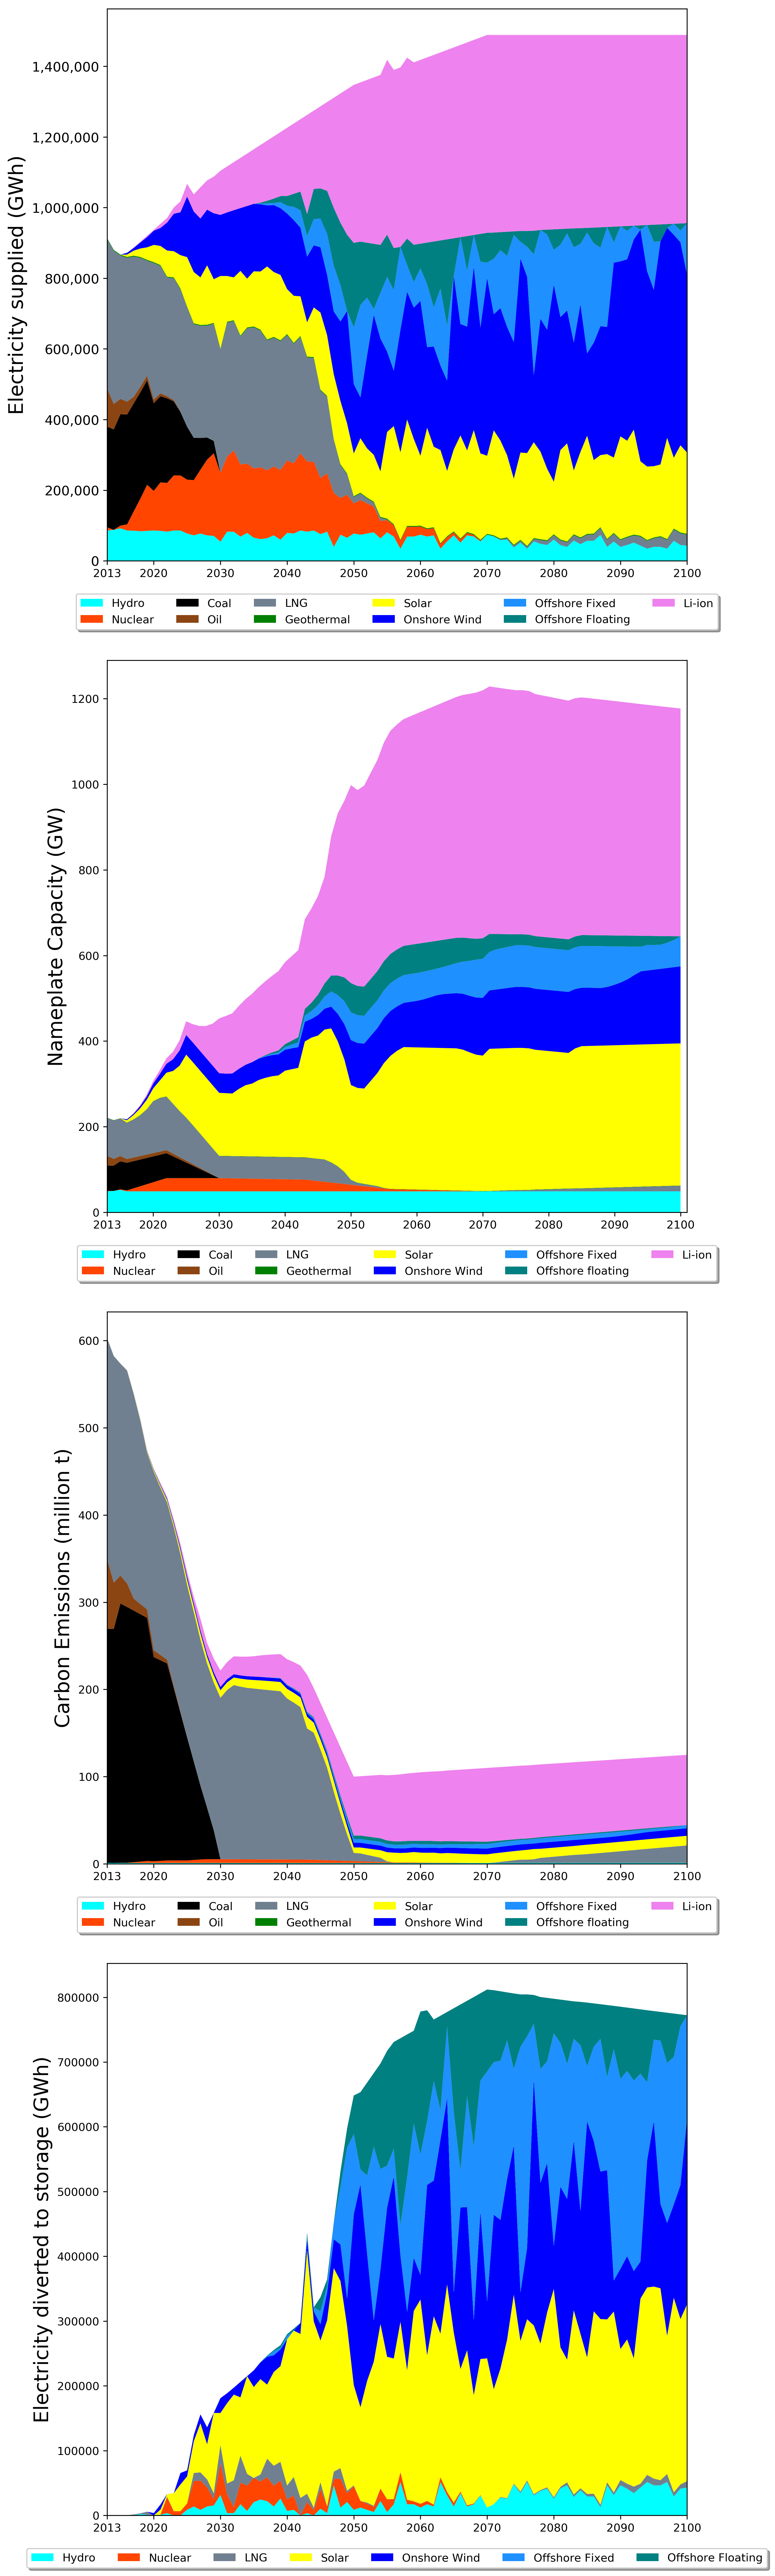
\includegraphics[scale=0.42]{figures/conv_nonuc}
\caption{Conventional technologies, no new nuclear.}
\label{scen1}
\end{figure}

\begin{figure}[h] 
\centering
\vspace*{-3cm}
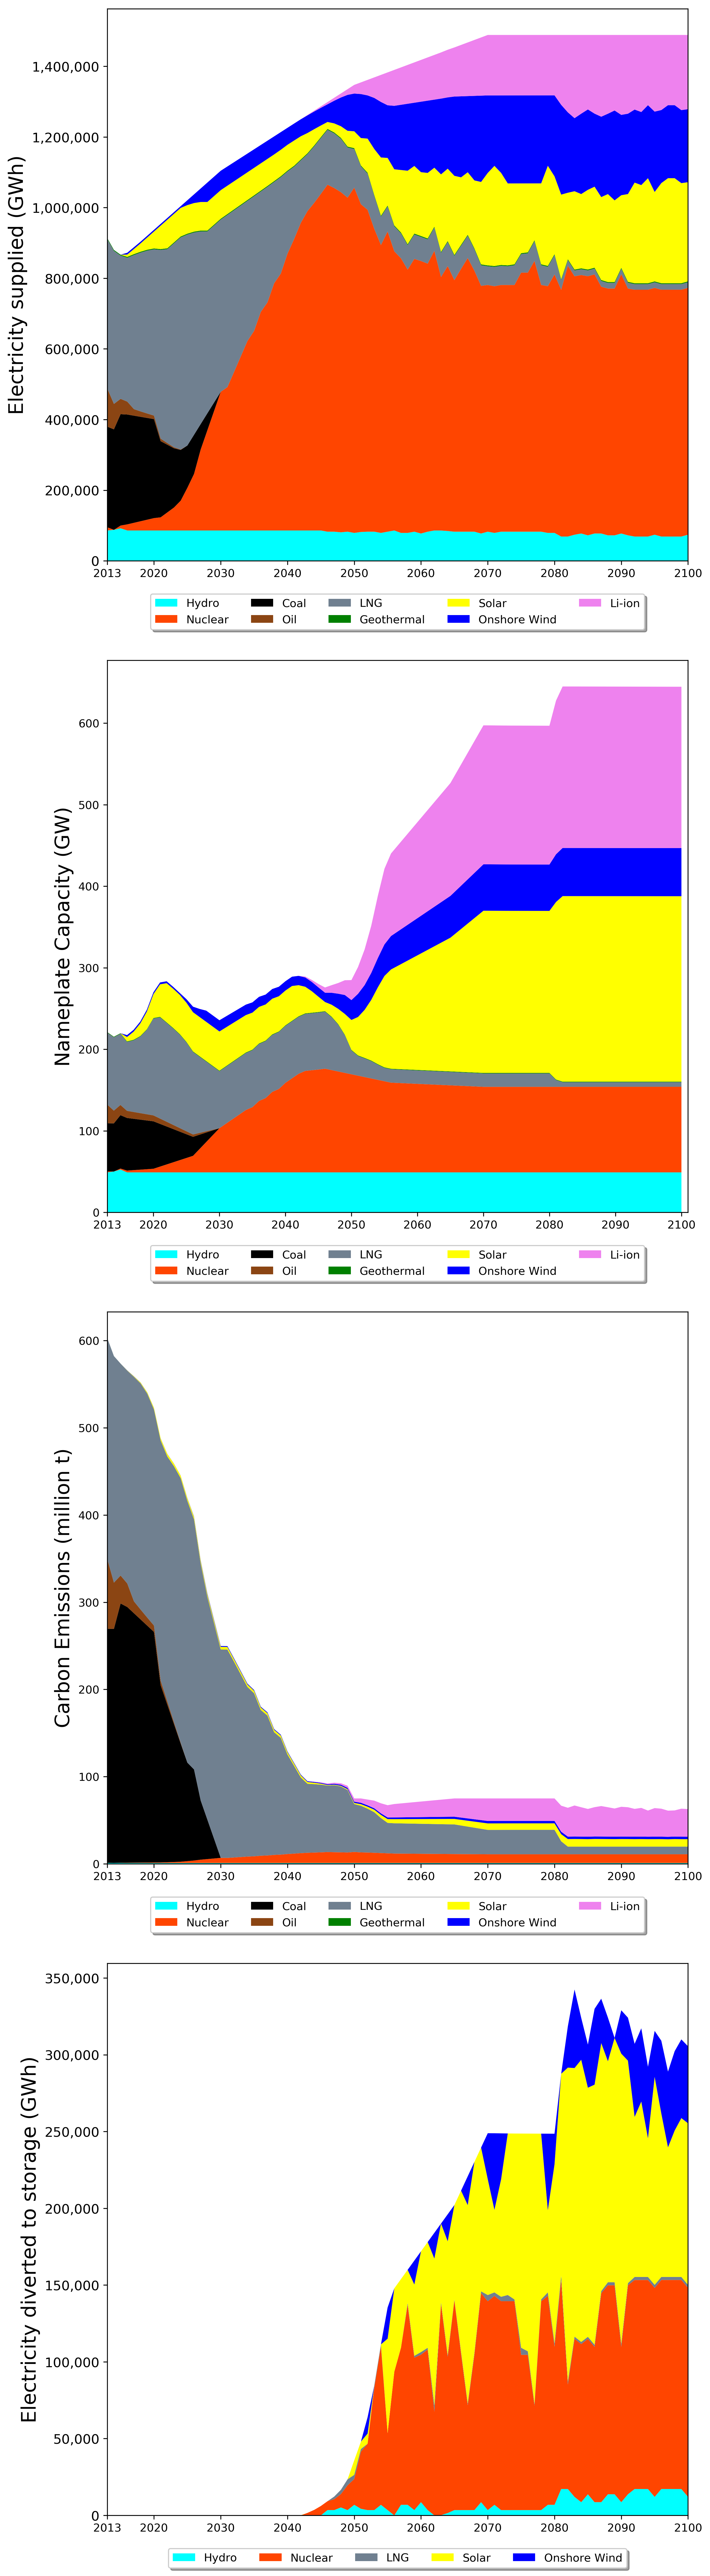
\includegraphics[scale=0.42]{figures/conv_nuc}
\caption{Conventional technologies, with new nuclear.}
\label{scen2}
\end{figure}

\begin{figure}[h] 
\centering
\vspace*{-3cm}
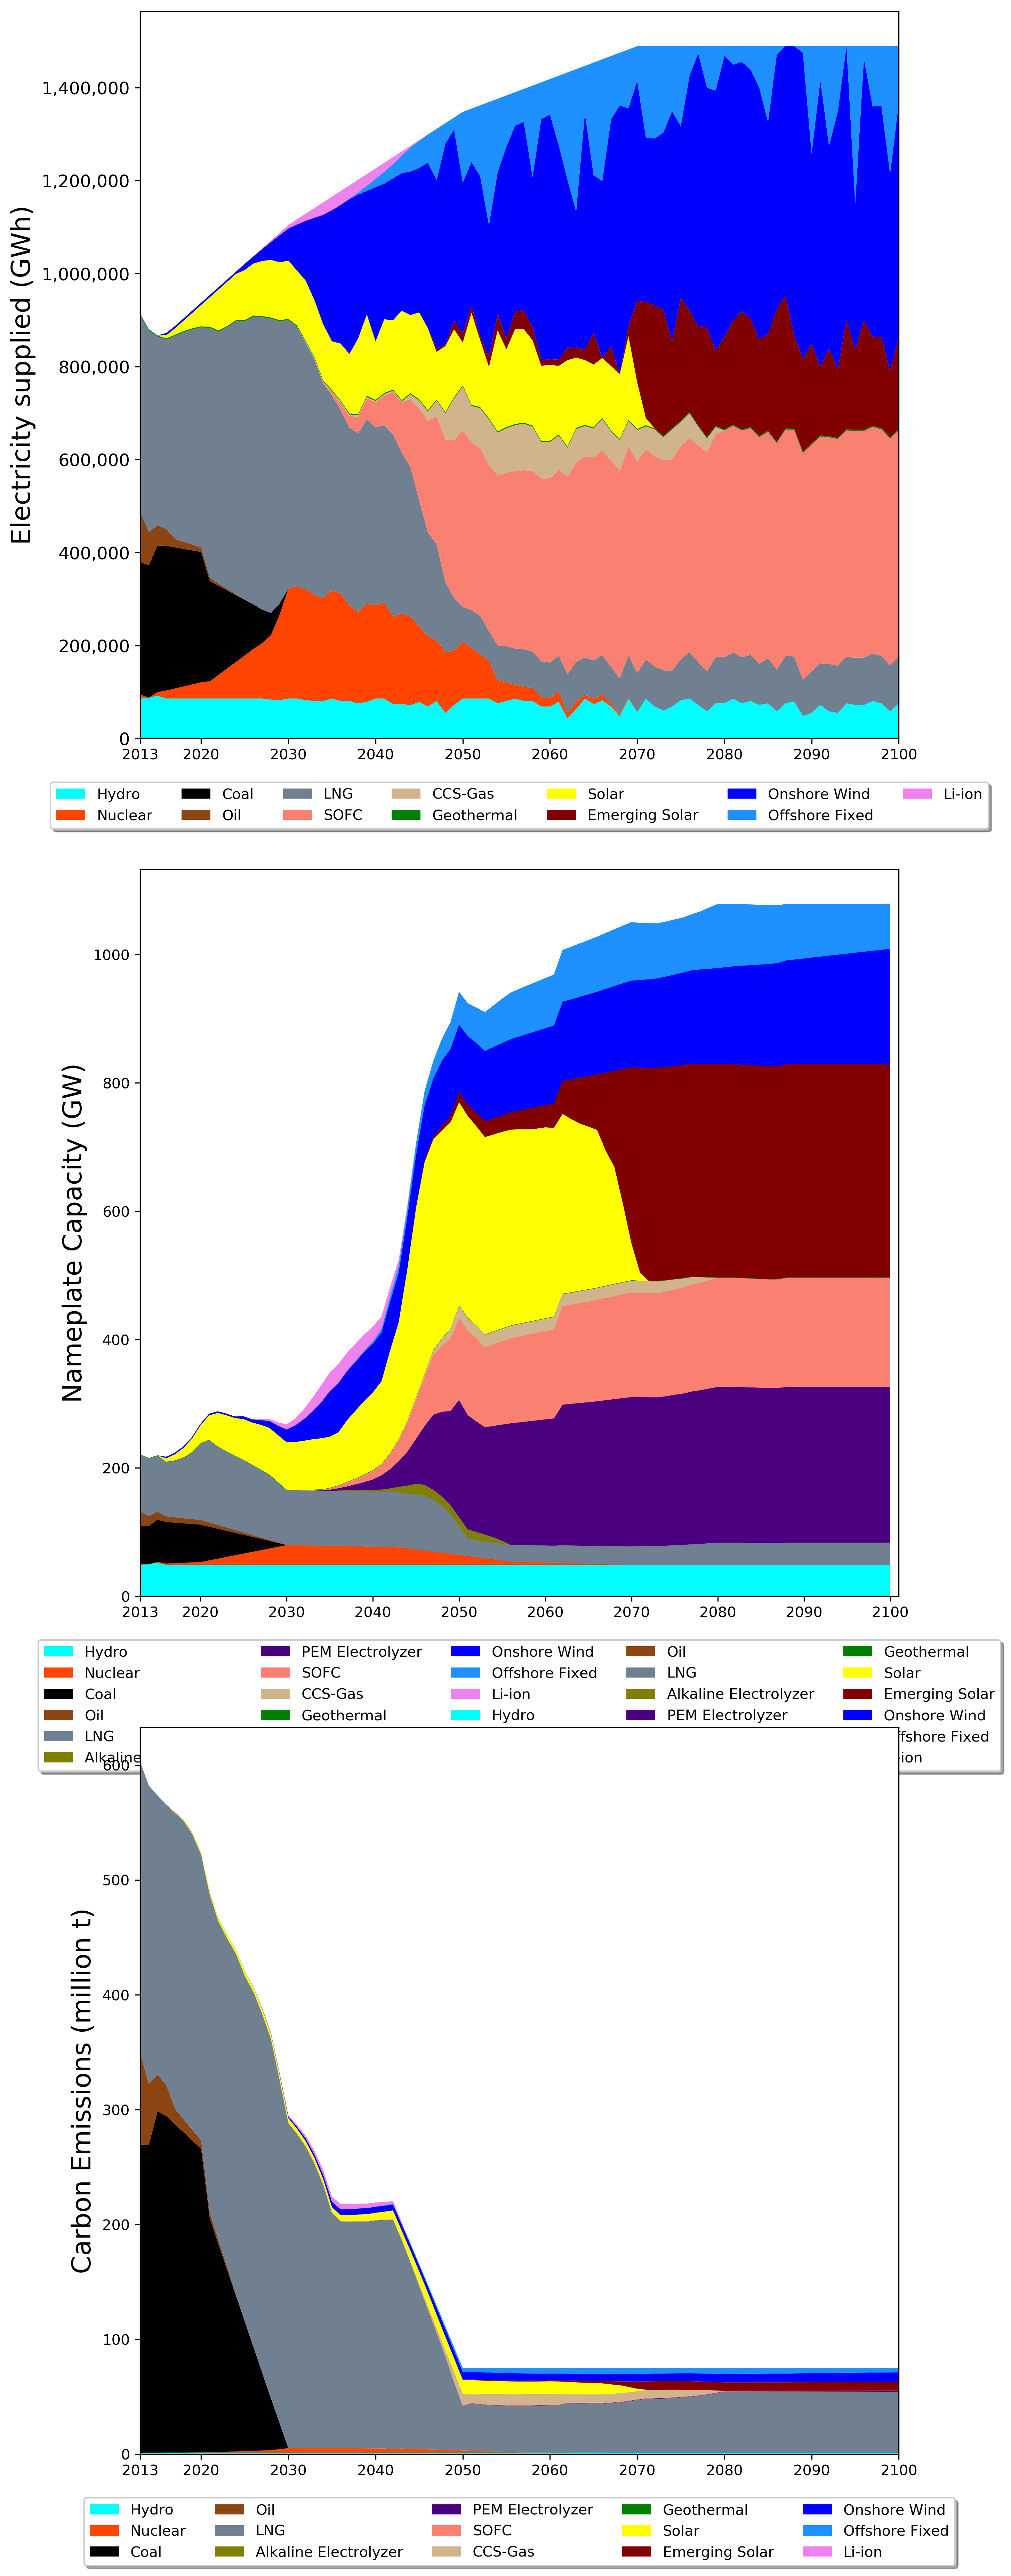
\includegraphics[scale=0.41]{figures/newtechs_nonuc}
\caption{Emerging technologies, no new nuclear.}
\label{scen3}
\end{figure}

\begin{figure}[h] 
\centering
\vspace*{-3cm}
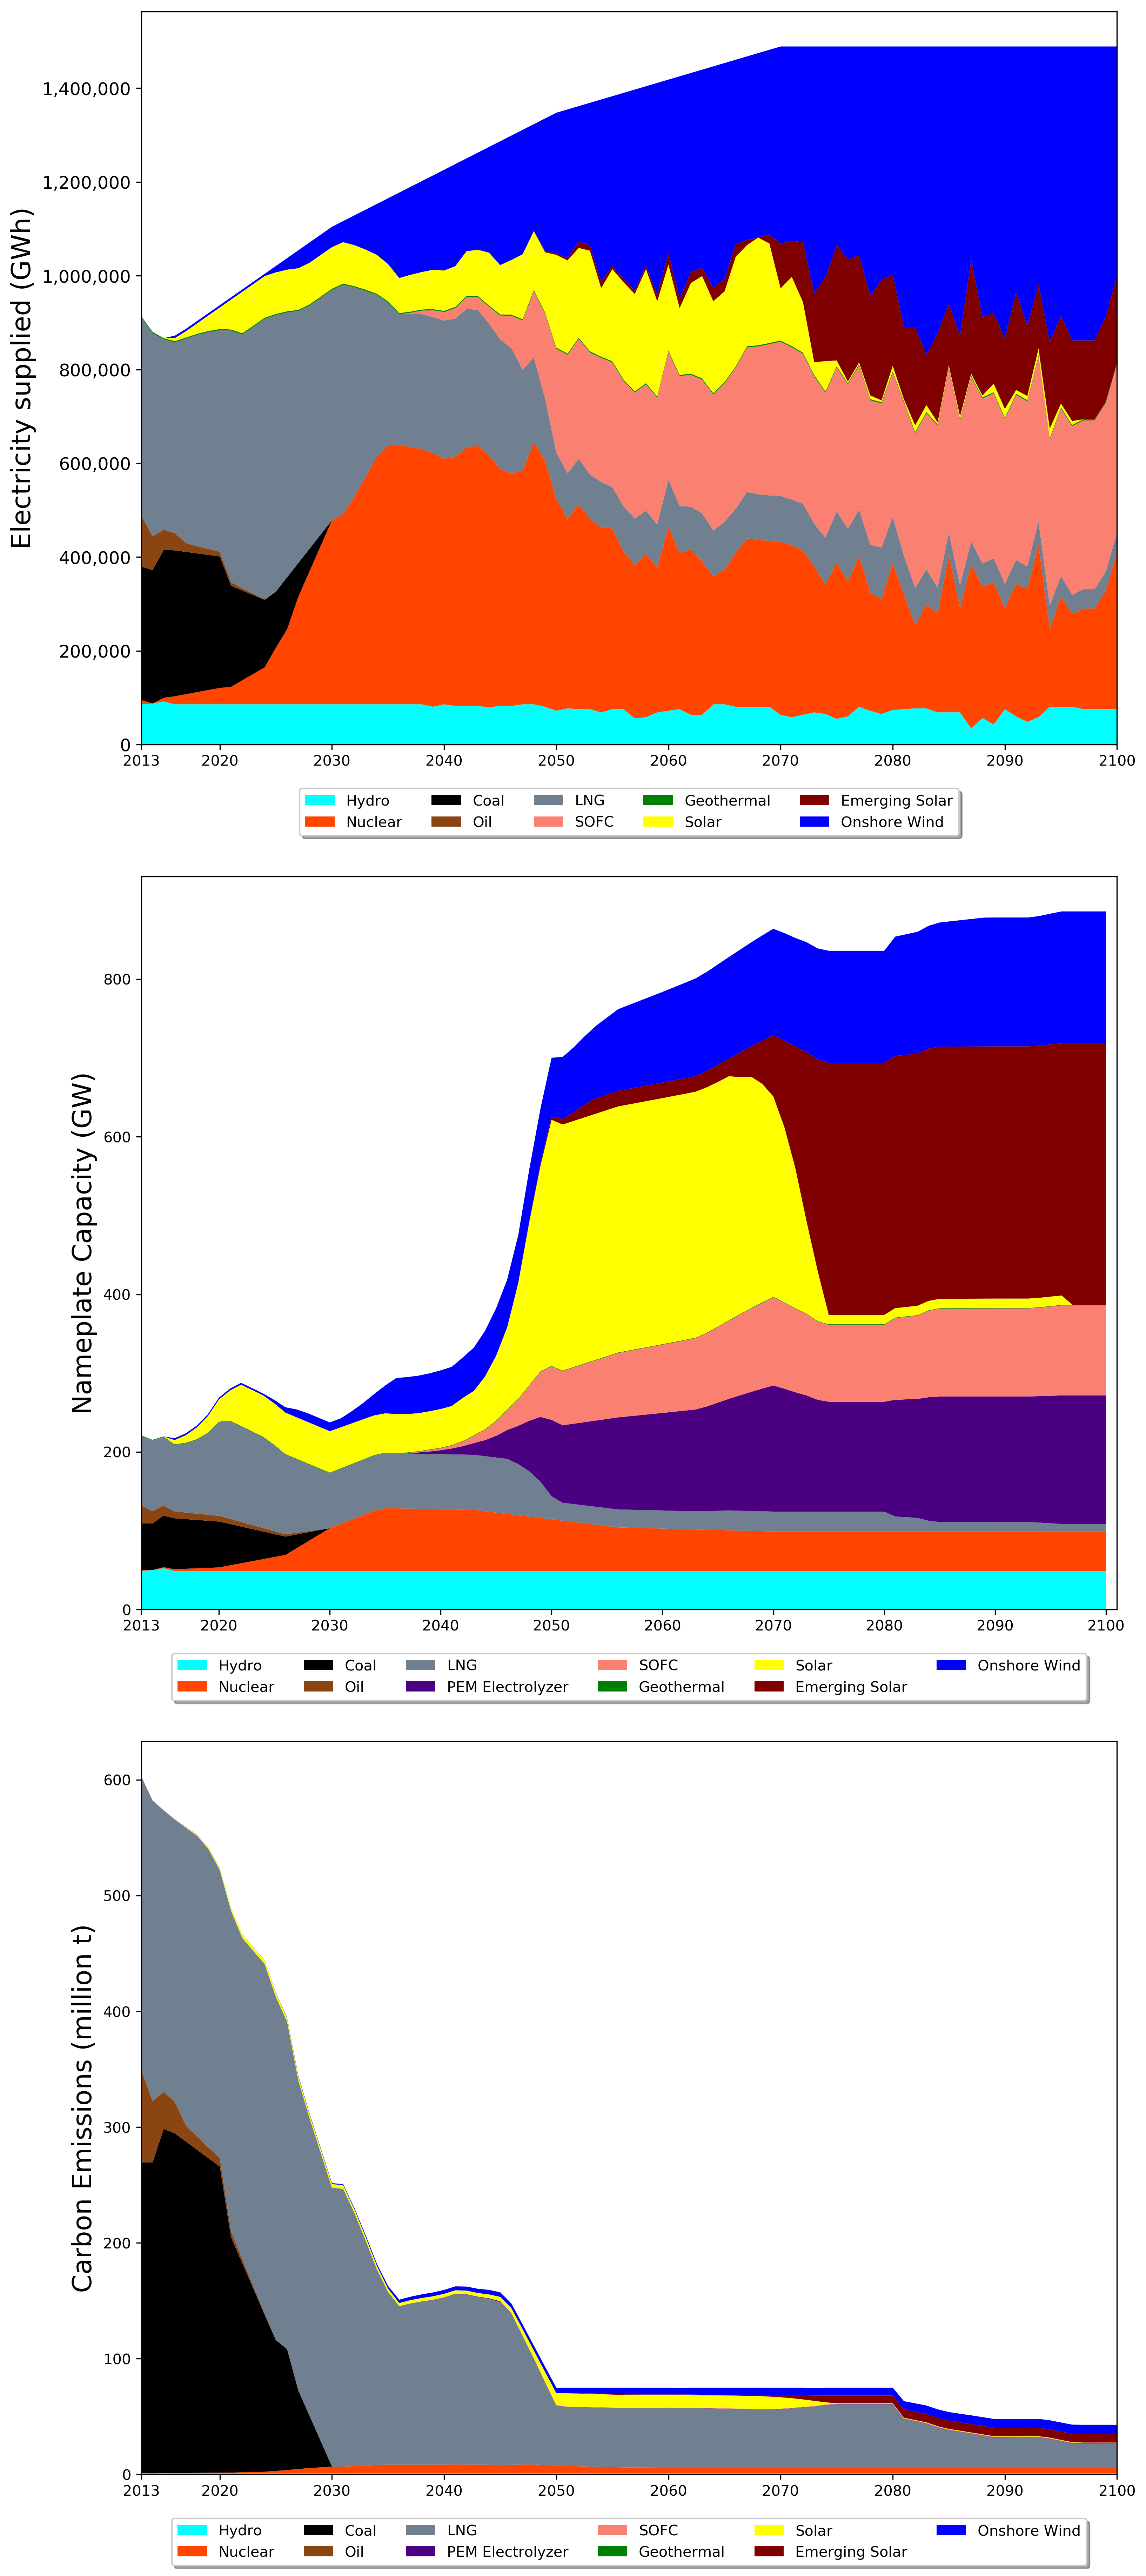
\includegraphics[scale=0.41]{figures/newtechs_nuc}
\caption{Emerging technologies, no new nuclear.}
\label{scen4}
\end{figure}

\subsection{Sensitivity analysis}